\documentclass{standalone}
% preamble: usepackage, etc.

\begin{document}
\chapter{The Capability of Convolution Neural Network}
\label{Chapter3}

For diverse applications, several deep learning algorithms have been thoroughly examined, allowing for pattern and attribute understanding for the interpretation of both basic and complex representations. In the field of machine vision and learning, substantial advancements have recently been made. The convolution Neural Network (CNN) has advanced into a strong tool for perceptual image processing and pattern understanding. The CNN framework effectively captures distinctive insights using learnable attributes via convolutions by mimicking the human visual brain. Similarly, wavelet convolution Neural Networks' ability to learn both spatial and spectral details from sequential data like signal and image has increased efficiency and made significant contributions to tasks like disease diagnosis, machine fault diagnosis, biometric authentication and verification, and so on. As a result, both CNN and wavelet multi-resolution analysis have been coupled in order to produce meaningful visual interpretation. This is mostly the combination of machine vision and wavelet function algorithms.

%%%%%%%%%%%%%%%%%%%%% Paper 2 %%%%%%%%%%%%%%%%%%%%%%%%%%%%%%%
\textbf{\section{The Capability of Wavelet Convolution Neural Network for Detecting Cyber Attack of Distribution Denial of Service n Smart Grid}}

In modern control systems, the term "smart grid" refers to a large-scale electricity distribution network. The smart grid's goal is to provide real-time power consumption control and analysis in order to increase device dependability, efficiency, and security while saving energy and money. Intelligent grids employ enhanced metering to offer two - way communications between intelligent meters and energy companies [1]-[3]. Although sophisticated measuring infrastructure is critical for intelligent grid communication due to its vulnerability to internet threats since adversaries can modify and deny data transfer, defeating the intelligent grid's objective. 

The distributed denial of service (DDoS) attack is a frequent type of internet attack [4], which can be expressly damaging since it delays, blocks, or corrupts smart grid communication [5]. As a consequence, this attack has the potential to disrupt power distribution, resulting in outages [4]. It's difficult to tell the difference between a DDoS attack and a normal burst signal. Both signals have hidden properties and are non-periodic, multi-fractal, broadband, self-affine, and stochastic. To differentiate between normal and abnormal signal behaviors, a heuristic automatic technique is required to extract signal properties. To get better outcomes, the majority of earlier approaches relied on shallow learning schemes or a mix of linear and non-linear approaches.
%%%%%%%%%%%%%%%%%%%%%%%%%%%%%%%%%%%%%%%%%%%%%%%%%%%% uncomment and insert your image
%\begin{figure*}[t!]
%\centering
%\includegraphics[scale=0.1]{pic/C3/c3_p2-1}
%\caption{Proposed scheme for detecting DDoS attack on smart grid.}
%\label{fig:c3_p2-1}
%\end{figure*}
This paper describes the procedure of our study in two phases. The first phase is to transform the one-dimensional time-series data to two-dimensional time-frequency scalogram as input image of distinct features with growing sensitivity using CWT which makes it suitable for CNN model. In the second phase, the image features obtained from CWT are utilized to train the proposed WavCovNet to detect attack and genuine traffic behaviors. 

\textbf{\subsection{Methodology}}
This section explains the proposed strategy for detecting DDoS attacks in intelligent grid infrastructure. The proposed approach for understanding the DDoS attack detection framework in the intelligent grid network is depicted in Figure 1. First, the dataset f or detecting DDoS attacks in intelligent grid infrastructure used in this dissertation is adequately defined.

\textbf{\subsubsection{Dataset}}
The first step is to collect both genuine and DDoS attack dataset. Setting up a real time network to generate large amounts of genuine and attack dataset is a difficult undertaking t hat necessitates a lot of network resources. Furthermore, establishing a large network takes time and money. However, one can avoid this time consuming task by utilizing a public network flow dataset. We chose the CICDDoS2019 dataset from a variety of public dataset [10] 10].
In comparison to numerous network traffic dataset, CICDDoS2019 [10] is the most recent dataset with a high number of contents. It also includes both incoming and outgoing traffic from recent DDoS attack.

\begin{figure*}[t!]
\centering
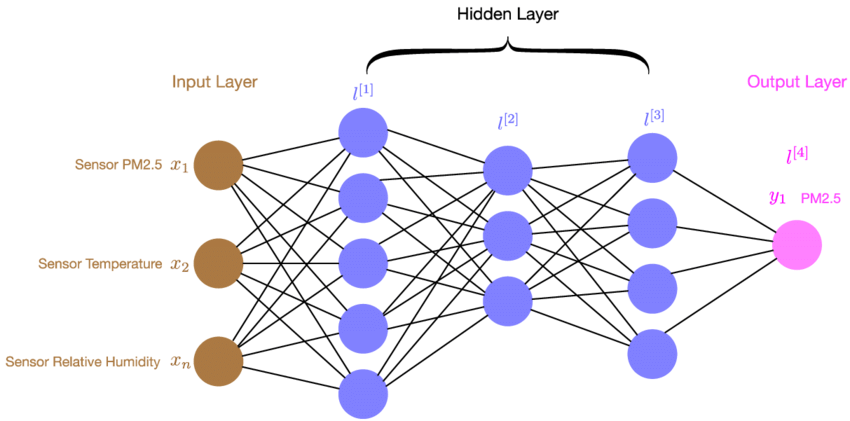
\includegraphics[scale=0.4]{pic/C3/c3_p2-2}
\caption{Adopting CWT for the Conversion of one-dimensional traffic data to two-dimensional scalogram.}
\label{fig:c3_p2-2}
\end{figure*}

\textbf{\subsubsection{Wavelet transform}}
Wavelet transform (WT) is a processing tool for extracting coefficients from a signal by using a wavelet function to turn it into wavelets [ 11]. WT decomposes data into coefficients and off er that information in sub scales. In this dissertation, we utilized continuous wavelet transform (CWT) for converting time series signal to time frequency images for detecting abnormalities in traffic patterns as depicted in Figure 2. {Equation \eqref{eq:2}} presents the mathematical expression for the CWT.

\begin{equation}
CWT_{x}^{\psi}= \frac{1}{\sqrt{|S|}} \int_{}^{}x(t) \psi^{*} (\frac{t-\tau}{S})dt 
\label{eq:2}
\end{equation}
where $\tau$ depicts the transition factor which is shift term to move the mother wavelet and $S$ denote the scale factor which is the frequency inverse. $x(t)$ represents the function of the mother wavelet. $\psi^{*} (\frac{t-\tau}{S})dt $ depicts the derived function from the mother wavelet. Low frequency corresponds to large S and small S leads to high frequency.


\textbf{\subsubsection{Convolution Neural Network}}

CNN is a sophisticated deep neural network based on visual perception that was first employed in the field of computer vision and has already shown great promise [12] 12]. CNN has recorded tremendous achievement in various applications especially detecting anomalies in radiographs [ 13]--[ 16]. With image as input, CNN may learn the hierarchical features to create a final set of high level
abstraction features, which are then sent to a fully connected layer as the classifier for categorical classification purposes. CNN learns the patterns in the images automatically and stores them in the network connection settings, requiring very little manual design. Furthermore, when compared to manual feature creation,
CNN is better at detecting intricate patterns in high dimensional data.




\textbf{\subsubsection{Proposed Wavelet Convolution Neural network}}

As shown in Figure 3 the proposed WavCovNet is a deep learning architecture that combines convolution layers in groups with wavelet decomposition layers generated from multi resolution analysis (MRA) f or DDoS attack detection . Two dimensional time frequency images with three channels are used as inputs to the proposed network. The resulting detail component from the first stage of decomposition is used as input to the first convolution
block, which is made up of two convolution layers.

After the approximate components of the first disintegration stage is further sub sampled to produce detail and approximate components of the second disintegration stage, the detail component of the first disintegration stage is fed as input to the second block, which comprises of two convolution network layers. It's worth mentioning that the detail component is concatenated through a channel of $1 \times 1$ convolution layer with a $64$ kernel size before being transferred to the second block to maintain a match in feature dimensionality with the output from the first block.

In the same fashion, the third and fourth blocks are treated same. At the third disintegration stage, the concatenation to the third block through the channel, on the other hand, is done via two $ 1 \times 1 $ convolution layers with kernel sizes of $64$  and $128$  respectively. The fourth block is made up of three convolution neural layers and average pooling, which is concatenated with the final decomposition level. Three $ 1 \times 1 $ convolution layers of $64$, $128$, and $256$ are used to achieve channel wise concatenation.



It's worth noting that the images are scaled down by a factor of two throughout the wavelet decomposition process. The fifth block is made up of two fully connected layers, and a classifier as the last fully connected layer with two class . We trained for $30$ epochs with a learning rate of $10^{4}$, $16$ as the batch size , and Adam as the optimizer. Training, validation, and test are the three sets of dataset split. During the training phase, the model's performance is also scrutinized. The suggested model is assessed using the test set split to obtain the final performance. Our model's performance was evaluated using well known metrics.

\textbf{\subsubsection{Experimental Detail and Setup}}

The core approach of the methodology is divided into two parts: data pre processing and feature extraction and learning. The raw DDoS data is transmitted to the network for the pre processing phase. Using digital signal processing met hods like CWT, the most significant and dependable underlying features are retrieved in the
pre processing step by converting the raw one dimensional traffic DDoS data to time frequency scalogram image data.


In this work, we trained our model for DDoS attack detection with continuous wavelet transform and wavelet convolutional neural network as a combined framework while using an Adam optimizer and dropout to avoid over fitting, early stop techniques is introduced and a learning rate of $10^{4}$ is used in order to obtain a better performance. We implemented the proposed model using Keras library with Tensorflow as back end on GeForce GTX 1080 GPU, which is driven by a parallel computing platform and programming paradigm called CUDA.

\textbf{\subsubsection{Performance Measures}}
We have applied some evaluation metrics in terms of accuracy, sensitivity, specificity and AUC on our proposed model. {Equation \eqref{eq:3}--\eqref{5}} are the numerical expression for the evaluation metrics.

\begin{equation}
Accuracy = \frac{TP+TN}{TP+TN+FP+FN}
\label{eq:3}
\end{equation}

\begin{equation}
Sensitivity = \frac{TP}{TP+FN}
\label{eq:4}
\end{equation}

\begin{equation}
Specificity = \frac{TN}{TN+FP}
\label{eq:5}
\end{equation}

\textbf{\subsection{Results and discussion}}
According to the automatic feature extraction method
depicted in {Figure \ref{fig:3}}, extensive experimental findings and discussion are presented in this section. The proposed attack detection system of DDoS is constructed on the Keras framework and utilizes Tensorflow as the back end. During the training and testing, we analyzed the proposed scheme for DDoS attack detection based on binary classification for both detecting and identifying incoming and outgoing DDoS attacks in smart grid networks. For detecting DDoS attacks, the proposed approach achieves 98.9\% accuracy.

\begin{table}[]
\caption{Performance comparison of our proposed model with selected pre-trained models.
WavCovNet model}
\label{tab5}
\begin{tabular}{lllll}
\toprule
\textbf{\multicolumn{1}{l}{Model}} & \textbf{\multicolumn{1}{l}{ACC (\%)}} & \textbf{\multicolumn{1}{l}{SEN (\%)}} & \textbf{\multicolumn{1}{l}{SPE (\%)}} & \textbf{\multicolumn{1}{l}{Time (Min)}} \\ \hline
\midrule
EfficientNet                & 95.1                         & 94.8                         & 95.2                         & 38                              \\
MobileNet V3                & 94.8                         & 95.4                         & 94.8                         & 41                              \\
DenseNet                    & 94.8                         & 95.7                         & 95.3                         & 51                              \\
ResNet 101                  & 94.6                         & 94.4                         & 95.8                         & 46                              \\\hline
\multicolumn{1}{l}{Ours}  & \multicolumn{1}{l}{98.9}    & \multicolumn{1}{l}{99.8}    & \multicolumn{1}{l}{99.9}    & \multicolumn{1}{l}{36}         \\ \hline
\bottomrule
\end{tabular}
\end{table}


{Figure \ref{fig:4}} depicts the training and validation accuracy curves of the proposed model which show that the model converges smoothly without over fitting. Figure 5 shows the gradual and steady reduction of the training and validation loss curves the proposed model. Generally, the performance of the proposed wavelet convolutional neural network is satisfactory. It is important to examine the validity of the proposed model in terms of the receiver operating characteristic curve (ROC) which shows the overall accuracy of the proposed scheme in terms of area under curve (AUC).


Figure 6 shows that the proposed model has high sensitivity associated with high specificity which minimizes the rate of false positive and maximizes the rate of true positive. Our proposed model achieves 99.8\% sensitivity and 99.9\% specificity as presented in Table 1. Table 1 shows the outcomes of our proposed methodology versus some pre-trained scheme. It is evident that the proposed technique outperformed the selected pre-trained methods by 3.8\% when it came to recognizing DDoS attack patterns in terms of accuracy. In addition, when compared to the pre-trained techniques, the proposed method obtained 3.2\% increase in sensitivity and a 3.1\% increase in specificity. ResNet-101 recorded the least score in accuracy (94.6\%) and sensitivity (94.4\%) whereas MobileNet-V3 recorded the least score in specificity (94.8\%). The proposed scheme is computational efficient with the least training time of 36 minutes as depicted in Table 1. Though DenseNet performed slightly better than ResNet-101, MobileNet-V3, and EfficientNet in accuracy, sensitivity, and specificity respectively but recorded the highest training time of 51 minutes for 30 epochs.

\textbf{\subsection{Conclusions}}

According to recent cyber-attack statistics, distributed denial of service (DDoS) attacks is the most common in smart grid infrastructure, and they are increasing in frequency and intensity over time. CNN models have acquired a lot of traction in image categorization applications as a result of their superior performance. However, CNN models are built to discover patterns in images therefore; they do not function as expected when trained on one-dimensional traffic data. In this paper, we proposed a method for converting a one-dimensional traffic data into two-dimensional time-frequency domain images in order to take advantage of CNN's potential. Following that, we trained our proposed WavCovNet on the converted data and evaluated its performance in recognizing DDoS attacks. The proposed approach detected DDoS attacks with 99.9\% accuracy, which is 9\% better than the pre-trained models. 


\end{document}
